

\vspace{-7mm}
This chapter gives routines for computing rotation matrices that operate on the expansion coefficients of spherical harmonics and spherical wave functions in order to rotate fields or view fields from a rotated frame.  The rotation matrices work the same for any of the wave functions in Chapter \ref{chap:wavefunctions}.

\section{Euler Rotation}
3D rotation of a Cartesian reference frame can be accomplished with three Euler angles $(\alpha,\beta,\gamma)$, where the sequence rotates the frame successively about one of its axes. The angles can take any value of radians. The most common rotation sequence is denoted Z-X'-Z'', sometimes just called ZXZ. This consists of a right-handed rotation of $\alpha$ about the $z$ axis, followed by a right-handed rotation of $\beta$ about the $x$ axis of the rotated frame (X'), followed by a right-handed rotation of $\gamma$ about the $z$ axis of the rotated frame (Z''). This is represented in a rotation matrix as:
\ea{
\bb{R}_{ZX'Z''}(\alpha,\beta,\gamma) &=& \bb{R}_{Z}(\alpha)\bb{R}_{X}(\beta)\bb{R}_{Z}(\gamma) \\
\ &= &
 \thbth{\cos(\alpha)}{-\sin(\alpha)}{0} {\sin(\alpha)}{ \cos(\alpha)}{ 0} {0}{ 0}{ 1}\thbth{1}{ 0}{ 0}{0 }{\cos(\beta)}{ -\sin(\beta)}{0}{ \sin(\beta) }{\cos(\beta)}\thbth{\cos(\gamma)}{ -\sin(\gamma)}{ 0} {\sin(\gamma)}{ \cos(\gamma) }{0}  {0 }{0 }{1} \label{rot}
}
Each matrix is a right-handed rotation about the axes of the unrotated, or fixed, global frame. The reason the matrices are applied in what seems like reverse order, and applied about the axes of the fixed frame, is because each matrix stacks the rotations in front of it to create the effect that each rotation was applied about the axes of the rotated frame in the order $(\alpha,\beta,\gamma)$.

\begin{figure}[H] 
   \centering
   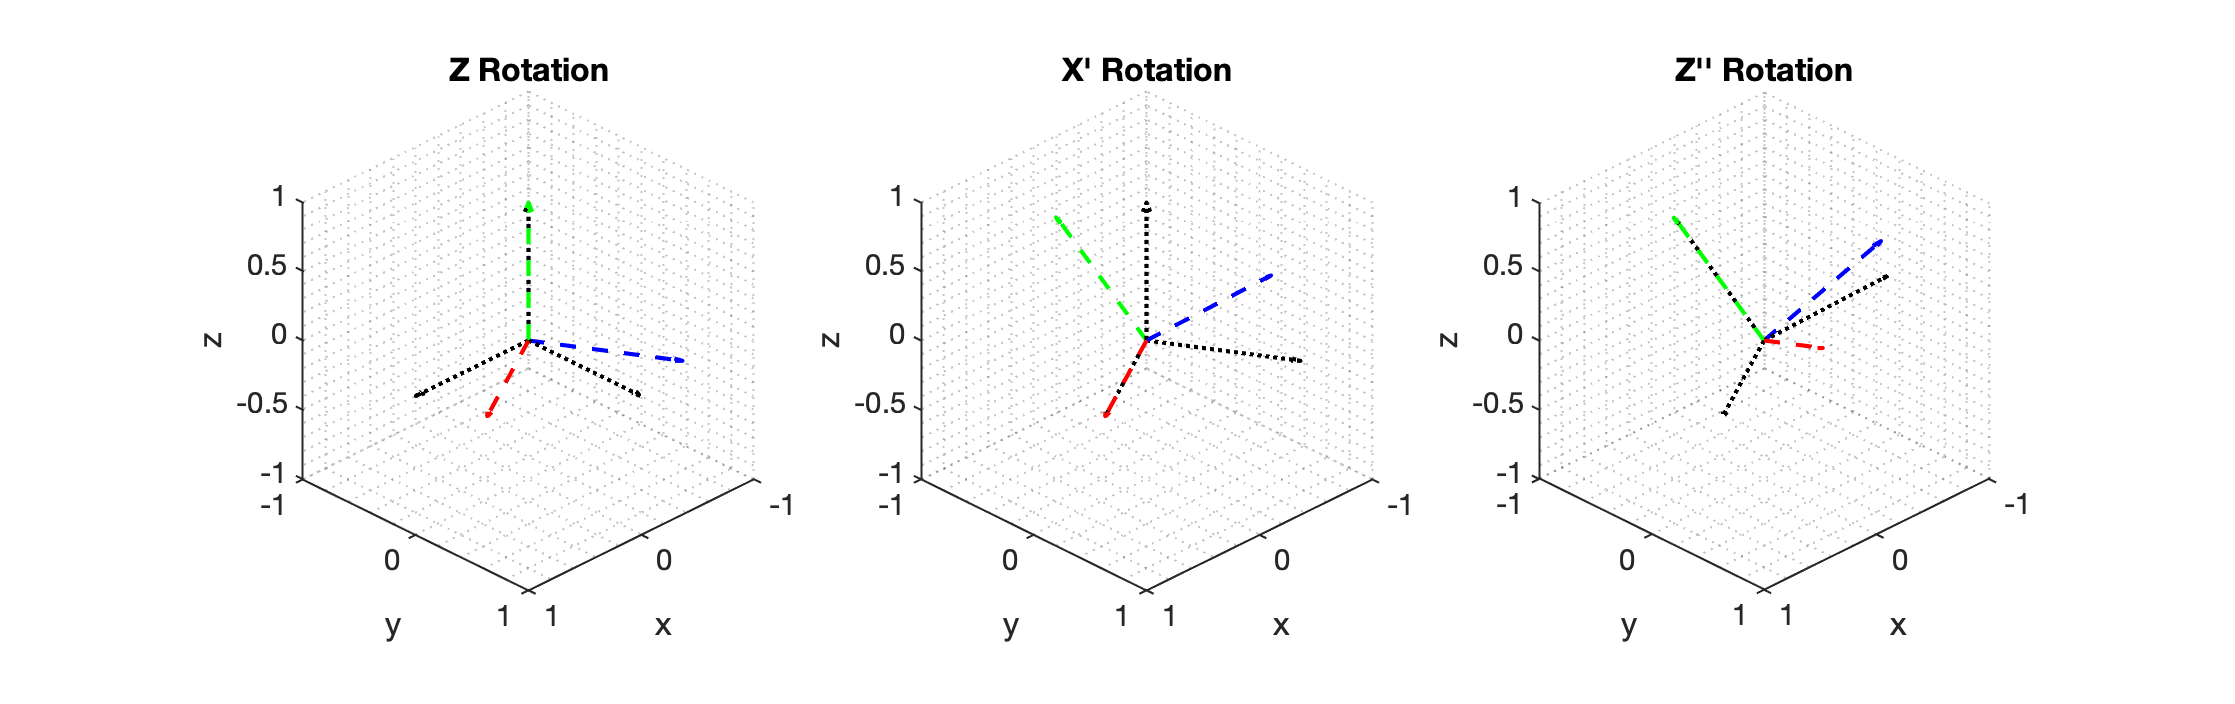
\includegraphics[width=6.5in]{Rotation/Figures/ZXZ} 
   \caption{ZX'Z'' rotation sequence $(\alpha,\beta,\gamma) = (\pi/6, \pi/5, \pi/4)$.  First pane shows the rotation of $\alpha$ about the $z$ axis from the original Cartesian frame (black dotted) to the new frame (red/blue/green). Second pane shows the second rotation of $\beta$ about the $x$ axis of the previously rotated frame. Third pane shows the final rotation of $\gamma$ about the $z$ axis of the previously rotated frame.}
   \label{fig1}
\end{figure}


A point $\bb{x} = [x, y, z]^t$ that in the global frame is rotated to the point $\bb{x}' = [x',y',z']^t$ as
\begin{equation}
\bb{x}' = \bb{R}\bb{x}
\end{equation}

\noindent In other words, the point is rotated through the global frame as though you are standing in the global frame. We call this a forward rotation. $\bb{R}$ is unitary, so the inverse is equal to the transpose, and 
\begin{equation}
\bb{x} = \bb{R}^t\bb{x}'
\end{equation}

The inverse rotation brings the point back, and applies the Euler angles in the reverse order and reverse direction. Given a forward set of angles $(\alpha,\beta,\gamma)$, applying the inverse is equivalent to fixing a point in the global frame and seeing it as you ride along with the rotating frame. We call this the inverse rotation.

Determining the ZXZ Euler angles from a rotation matrix is done with 
\begin{eqnarray}
\alpha & =& \arctan \dfrac{R_{13}}{-R_{23}} \\
\beta & =& \arctan \dfrac{\sqrt{R_{13}^2 + R_{23}^2} }{R_{33}}\\
\gamma &=& \arctan \dfrac{R_{31}}{R_{32}} 
\end{eqnarray}

\noindent where $R_{ij}$ are the matrix entries of $\bb{R}$. 

The rotation matrix and Euler angle conversions are given in the routines \texttt{euler2rot} and \texttt{rot2euler}. A plotting function,  \texttt{plotrot}, not copied here, will plot the axes of the rotated frame given $\bb{R}$. 

{\footnotesize
\VerbatimInput{\code/Rotation/euler2rot.m}
}

{\footnotesize
\VerbatimInput{\code/Rotation/rot2euler.m}
}

%{\footnotesize
%\VerbatimInput{\code/Rotation/plotrot.m}
%}



\clearpage
\section{Rotation Addition Theorem}

The rotation addition theorem for spherical harmonics is given by  
\begin{equation}
Y_{lm}(\theta,\phi) = \sum_{p=-l}^{l} D_{lmp}(\alpha,\beta,\gamma) Y_{lp}(\theta',\phi')
\end{equation}

\noindent where $(\alpha,\beta,\gamma)$ are the three Euler angles describing a ZXZ rotation from unprimed to primed coordinate systems. $D_{lmp}$ is the rotation matrix for spherical harmonics. Because the coordinate $r$ and the gradient are invariant under rotation, the rotation addition theorem for scalar and vector wave functions have identical forms \cite{edmonds1996angular,hansen1988spherical,stein1961addition,dufva2008unified},
\begin{equation}
\psi_{lm}(r,\theta,\phi) = \sum_{p=-l}^{l} D_{lmp}(\alpha,\beta,\gamma) \psi_{lp}(r',\theta',\phi')
\end{equation}
\begin{equation}
\bb{M}_{lm}(r,\theta,\phi) = \sum_{p=-l}^{l} D_{lmp}(\alpha,\beta,\gamma)\bb{M}_{lp}'(r',\theta',\phi')
\end{equation}

This means that the same $D_{lmp}$ can be used to rotate any of following: spherical harmonics, scalar spherical wave functions, vector spherical harmonics, or vector spherical wave functions. $D_{lmp}$ is a square block diagonal matrix with blocks that span $m$ and $p$ for a given $l$, zero otherwise.  Specifically,
\begin{equation}
D_{lmp}(\alpha,\beta,\gamma) = e^{im\alpha}d_{lmp}(\beta)e^{ip\gamma} \label{dlmpsep}
\end{equation}

The rotation matrix is inherently separable in $(\alpha,\beta,\gamma)$, where $\alpha$, and $\gamma$ are diagonal. The matrix $d_{lmp}(\beta)$, called "little-d", is block diagonal and can be computed itself. This is advantageous when precomputing rotation matrices over many combinations of Euler angles. The matrix $d_{lmp}(\beta)$ is given by 
\begin{eqnarray}
d_{lmp}(\beta) &=&  i^{m-p}\sqrt{\dfrac{(l+p)!(l-p)!}{(l+m)!(l-m)!}} \sum_s (-1)^{s}  {l+m \choose l+p-s} {l-m \choose s}  \left(\cos\frac{\beta}{2}\right)^{2l+p-m-2s}\left(\sin\frac{\beta}{2}\right)^{m-p+2s}  \label{dlmpdirect}
\end{eqnarray}


The sum is over all $s$ for positive arguments of the binomial coefficients. There is a version used in quantum mechanics, \cite{wigner2012group}, based on a ZYZ rotation that yields a real-valued $d_{lmp}(\beta)$ matrix. This forms the basis of a recursion algorithm in Section \ref{littled}. The mapping from complex ZXZ  $d_{lmp}(\beta)$ to the purely real ZYZ is, \cite{littledconversion},
\eq{ d_{lmp}^{ZYZ}(\beta)   =  (-i)^{p-m} d_{lmp}^{ZXZ}(\beta)   \label{zyzzxzconv} }
%\eq{ d_{lmp}^{ZYZ}(\beta)   = i^{p-m} (-1)^{p-m} d_{lmp}^{ZXZ}(\beta)   \label{zyzzxzconv} }



%
%\begin{eqnarray}
%d_{lmp}(\beta) &=&  \sqrt{\frac{(l+p)!(l-p)!}{(l+m)!(l-m)!}}\sum_u {l+m \choose l-p-u}{l-m \choose u} \nonumber \\
%\ & \ & \cdot (-1)^{l-p-u}\left(\cos\frac{\beta}{2}\right)^{m+p+2u}\left(\sin\frac{\beta}{2}\right)^{2l-m-p-2u} 
%\end{eqnarray}
%
%The sum is over all $u$ for positive arguments of the binomial coefficients.  


%From Wikipedia ("Wigner-D Matrix"), the rotation matrix is given as
%\eq{D_{lmp}(\alpha\beta\gamma) = e^{-im\alpha}d_{lmp}(\beta)e^{-ip\gamma}}
%
%with 
%\begin{eqnarray}
%d_{lmp}(\beta) &=&  \sqrt{(l+m)!(l-m)!(l+p)!(l-p)!} \sum_s  \dfrac{(-1)^{m-p+s}}{(l+p-s)!s!(m-p+s)!(l-m-s)!} \nonumber \\
%\ & \ & \cdot  \left(\cos\frac{\beta}{2}\right)^{2l+p-m-2s}\left(\sin\frac{\beta}{2}\right)^{m-p+2s} 
%\end{eqnarray}

%\begin{eqnarray}
%d_{m'm}^j(\beta) &=&  \sqrt{(j+m')!(j-m')!(j+m)!(j-m)!} \sum_s  \dfrac{(-1)^{m'-m+s}}{(j+m-s)!s!(m'-m+s)!(j-m'-s)!} \nonumber \\
%\ & \ & \cdot  \left(\cos\frac{\beta}{2}\right)^{2j+m-m'-2s}\left(\sin\frac{\beta}{2}\right)^{m'-m+2s} 
%\end{eqnarray}
%
%This is for a ZYZ rotation, which results in the purely real $d_{lmp}$.  For ZXZ Euler rotations, the $(-1)^{m-p+s}$ is replaced with $(-1)^s i^{p-m}$ and $s$ runs from $[0,l+p]$ while for valid factorials.  However, I found that $(-1)^s i^{m-p}$ and multiplying the diagonal matrices in reverse (conjugate transpose) as $e^{im\gamma}d_{lmp}(\beta)e^{ip\alpha}$ matched the values given by the recursion algorithm above. Therefore, the transform between the purely real and complex  $d_{lmp}(\beta)$ is 
%\eq{ d_{lmp}(\beta) \leftarrow i^{m-p} (-1)^{m-p} d_{lmp}(\beta)}
%


%\begin{eqnarray}
%d_{lmp}(\beta) &=&  \sqrt{(l+m)!(l-m)!(j+p)!(j-p)!} \sum_s  \dfrac{(-1)^{m-p+s}}{(l+p-s)!s!(m-p+s)!(l-m-s)!} \nonumber \\
%\ & \ & \cdot  \left(\cos\frac{\beta}{2}\right)^{2l+p-m-2s}\left(\sin\frac{\beta}{2}\right)^{m-p+2s}  \\
%\ &=&  \sqrt{\dfrac{(l+p)!(l-p)!}{(l+m)!(l-m)!}} \sum_s  \dfrac{(-1)^{m-p+s} (l+m)!(l-m)! }{(l+p-s)!s!(m-p+s)!(l-m-s)!}   \left(\cos\frac{\beta}{2}\right)^{2l+p-m-2s}\left(\sin\frac{\beta}{2}\right)^{m-p+2s}  \\
%\ &=&  \sqrt{\dfrac{(l+p)!(l-p)!}{(l+m)!(l-m)!}} \sum_s (-1)^{m-p+s}  {l+m \choose l+p-s} {l-m \choose s}  \left(\cos\frac{\beta}{2}\right)^{2l+p-m-2s}\left(\sin\frac{\beta}{2}\right)^{m-p+2s} 
%\end{eqnarray}




\subsection{Field Rotations} 

Given a field expansion in an unprimed system, 
\begin{equation}
\bb{E}(\bb{r}) = \sum_{lm}a_{lm}\bb{M}_{lm}(k,\br)+b_{lm}\bb{N}_{lm}(k,\br)
\end{equation}

the expansion coefficients in the primed system are found by substituting the addition theorem 

\begin{equation}
\bb{E}'(\bb{r}') = \sum_{lp}a_{lp}'\bb{M}_{lp}'(k,\br')+b_{lp}'\bb{N}_{lp}'(k,\br')
\end{equation}

\noindent where 

\begin{equation}
a_{lp}' = \sum_m a_{lm}D_{lmp}, \quad \quad
b_{lp}' = \sum_m b_{lm}D_{lmp}
\end{equation}

In matrix form, if $\bb{a}$ are the outgoing wave coefficients in the $i$ frame, and $\bb{a}'$ are those in the rotated $i'$ frame, then 
\begin{equation}
\bb{a}' = \bb{D}_i\bb{a}
\end{equation}

\noindent where $\bb{D}_i$ is the rotation matrix, and $(\alpha,\beta,\gamma)$ describe the rotation from $i$ to $i'$.  In other words, the application of $\bb{D}_i$ is an inverse rotation on the field (the coefficients $\bb{a}'$ describe the same field but viewed from the rotated frame). $\bb{D}_i$ is unitary, so the inverse is the conjugate transpose: $\bb{D}_i^{-1} = \bb{D}^*_i$.  This is the forward rotation, where the field itself rotates, to follow the Euler angles, as seen from the originating frame. 

%, and the inverse relation is 
%
%\begin{equation}
%\bb{a} = \bb{D}^*_i\bb{a}'
%\end{equation}


\subsection{Properties} 

Here we give several properties of the rotation matrix. The transpose satisfies the following relation
\eq{D_{lmp}(\alpha,\beta,\gamma) = D_{lpm}^*(-\gamma+\pi,\beta,-\alpha+\pi) }
The following relation exists for conjugated matrix elements
\eq{D_{l,-m,-p} = (-1)^{m+p}D_{lmp}^*}

The following identity exists between the $d_{lmp}(\beta)$ and the Legendre polynomials
\ea{d_{l00}(\beta) &=& P_l(\cos\beta) }

The rotation matrix is orthogonal over the three Euler angles as
\eq{\int_{0}^{2\pi} \int_{0}^{\pi} \int_{0}^{2\pi} D_{l'm'p'}^*(\alpha,\beta,\gamma) D_{lmp}(\alpha,\beta,\gamma) d\alpha \sin\beta d\beta d\gamma
= \dfrac{8 \pi^2}{2 l + 1} \delta_{l'l}\delta_{m'm}\delta_{p'p}}

where 
\eq{\int_{0}^{2\pi}  d\alpha \int_{0}^{\pi} \sin\beta d\beta  \int_{0}^{2\pi} d\gamma
= 8 \pi^2}

The same integral computed over a matrix element is 
\ea{I_{lmp} &=& \int_{0}^{2\pi} \int_{0}^{\pi} \int_{0}^{2\pi} D_{lmp}(\alpha,\beta,\gamma) d\alpha \sin\beta d\beta d\gamma \\
\ &=& 4\pi^2 \delta_{m,0}  \delta_{p,0} \int_{0}^{\pi}d_{lmp}(\beta) \sin\beta d\beta  \\
\ &=& 4\pi^2 \delta_{m,0}  \delta_{p,0}\int_{0}^{\pi}P_l(\cos\beta) \sin\beta d\beta  \\ 
\ &=& 8 \pi^2 \delta_{l,0}\delta_{m,0}  \delta_{p,0} }

For $\alpha = 0$, $\gamma = 0$, the sum over the diagonal elements of the blocks satisfy
\eq{\sum_{m=-l}^l D_{lmm}(\beta) = \sum_{m=-l}^l d_{lmm}(\beta) = \dfrac{\sin\left(\dfrac{(2 l+1)}{2}\beta\right)}{\sin\left(\dfrac{\beta}{2}\right)}}

which is the normalized Dirichlet kernel.  



\clearpage
\newpage

\section{Computation of $D_{lmp}$}

Direct computation of the rotation matrix using \eqref{dlmpsep} and \eqref{dlmpdirect} is not advised because of the need to compute the binomial coefficients. Instead, a fast recursion algorithm for computing the full $D_{lmp}$ is given in \cite{choi1999rapid}. This begins with a rotation matrix defined
\begin{equation}
(\hat{x},\hat{y},\hat{z}) = (x,y,z)\thbth{R_{xx}}{R_{xy}}{R_{xz}}{R_{yx}}{R_{yy}}{R_{yz}}{R_{zx}}{R_{zy}}{R_{zz}} = (x,y,z)\bb{R}
\end{equation}

which is opposite to the rotation matrix in \eqref{rot}. Next, \cite{choi1999rapid} defines the following matrices 
\begin{equation}
\bb{D} = \bb{F} + i\bb{G}
\end{equation}
\begin{equation}
\bb{F} = \thbth{(R_{yy}+R_{xx})/2}{R_{xz}/\sqrt{2}}{(R_{yy}-R_{xx})/2}{R_{zx}/\sqrt{2}}{R_{zz}}{-R_{zx}/\sqrt{2}}{(R_{yy}-R_{xx})/2}{-R_{xz}/\sqrt{2}}{(R_{yy}+R_{xx})/2}
\end{equation}
\begin{equation}
\bb{G} = \thbth{(R_{yx}-R_{xy})/2}{R_{yz}/\sqrt{2}}{-(R_{yx}+R_{xy})/2}{-R_{zy}/\sqrt{2}}{0}{-R_{zy}/\sqrt{2}}{(R_{yx}+R_{xy})/2}{R_{yz}/\sqrt{2}}{(R_{xy}-R_{yx})/2}
\end{equation}

\noindent which serves as the initial condition
\eq{D_{1mp} = \bb{D}}
%\begin{eqnarray}
%D_{lmp} &=& F_{lmp} + iG_{lmp} \\
%\bb{D}_{1mp} &=& \bb{D}
%\end{eqnarray}

The recursion equations are given as follows: 
\begin{enumerate}
\item For $(-l+1) \leq p \leq (l-1)$:
\begin{equation}
D_{lmp} = a_{lmp}D_{100}D_{l-1,mp}+b_{lmp}D_{110}D_{l-1,m-1,p}+b_{l,-m,p}D_{1,-10}D_{l-1,m+1,p}
\end{equation}
\begin{eqnarray}
a_{lmp} &=& \sqrt{\frac{(l+m)(l-m)}{(l+p)(l-p)}} \\
b_{lmp} &=& \sqrt{\frac{(l+m)(l+m-1)}{2(l+p)(l-p)}} 
\end{eqnarray}
$p = \pm l$ is not covered, $a_{lmp} = 0$ for $m=\pm l$, and $b_{lmp} = 0$ for both $m=-l$ and $m=-l+1$.

\item For $-l \leq p \leq (l-2)$:
\begin{eqnarray}
D_{lmp} &=& c_{lm,-p}D_{10,-1}D_{l-1,m,p+1}+d_{lm,-p}D_{11,-1}D_{l-1,m-1,p+1} \nonumber \\
\ & \ & +d_{l,-m,-p}D_{1,-1,-1}D_{l-1,m+1,p+1}
\end{eqnarray}
\begin{eqnarray}
c_{lmp} &=& \sqrt{\frac{2(l+m)(l-m)}{(l+p)(l+p-1)}} \\
d_{lmp} &=& \sqrt{\frac{(l+m)(l+m-1)}{(l+p)(l+p-1)}} 
\end{eqnarray}
$p = \pm l$ and $p=(l-1)$ are not covered, $c_{lmp} = 0$ for $m=\pm l$, and $d_{lmp} = 0$ for both $m=-l$ and $m=-l+1$.

\item For $(-l+1) \leq p \leq l$:
\begin{eqnarray}
D_{lmp} &= &c_{lm,p}D_{101}D_{l-1,m,p-1}+d_{lm,p}D_{111}D_{l-1,m-1,p-1} \nonumber \\
\ & \ & +d_{l,-m,p}D_{1,-1,1}D_{l-1,m+1,p-1}
\end{eqnarray}
$p = -l$ and $p = -l+1$ are not covered, and $c_{lmp}$ and $d_{lmp}$ are the same as above.
\end{enumerate}

This algorithm is the basis for two routines that follow. The first routine computes \texttt{Dlmp} on a full square matrix, which has mostly zero elements. The second routine is specialized to compute this on a sparse 1D array to same memory.  

\subsection{Full $D_{lmp}$ Matrix}

The routine \texttt{Dlmp} returns the rotation matrix in full, including zeros, starting with $l=1$. As mentioned, this describes an inverse rotation. Use the string switch \texttt{'mono'} to include the monopole term. The algorithm above uses a rotation matrix that is transposed from our convention, so we transpose it on input to keep the routine consistent. There are helper functions to compute the coefficients: \texttt{a\_lmp}, \texttt{b\_lmp}, \texttt{c\_lmp}, \texttt{d\_lmp}.  Figure \ref{fig1} shows the magnitude of $D_{lmp}$ for different $\beta$ ($\alpha$, $\gamma$ do not affect the magnitude).  

\begin{figure}[H] 
   \centering
   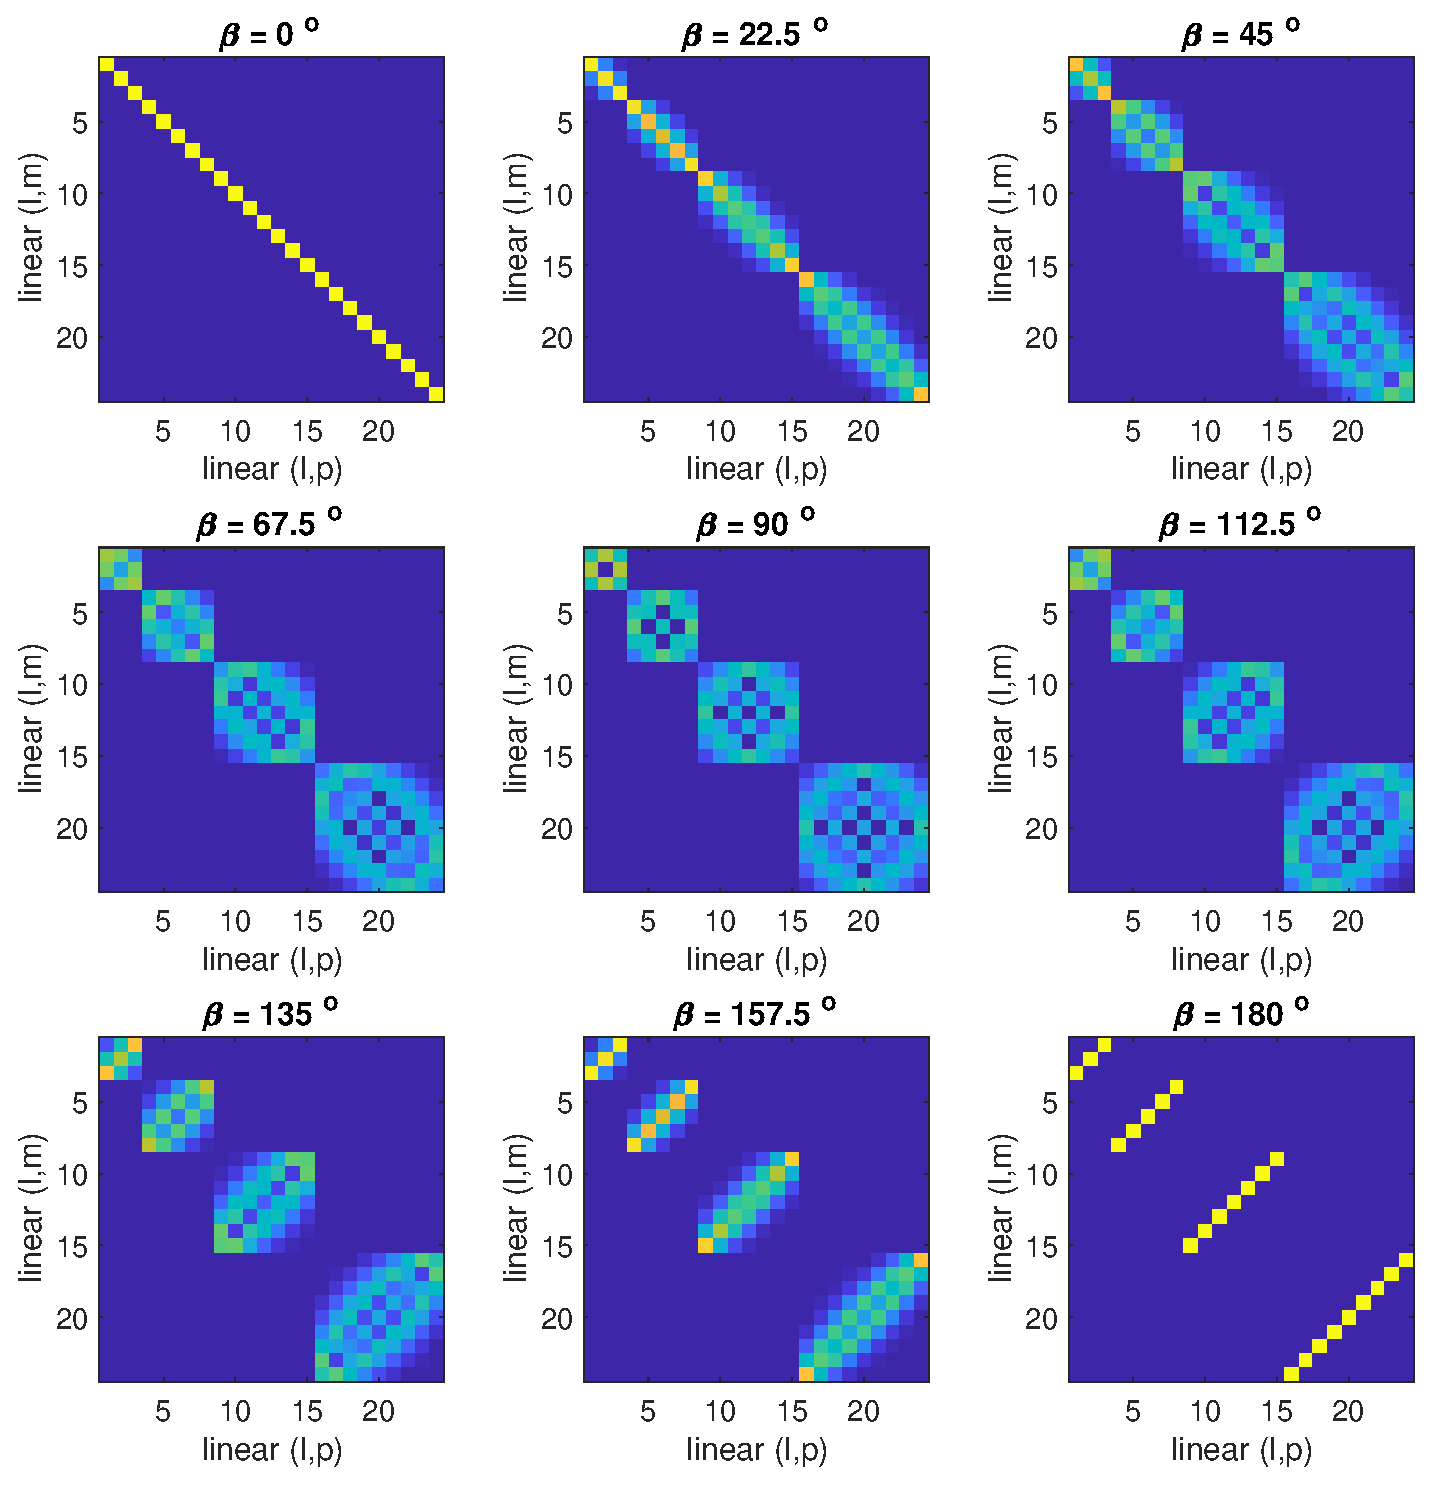
\includegraphics[width=4in]{Rotation/Figures/Dlmp} 
   \caption{$D_{lmp}$ magnitude (color scale [0, 1]) for varying $\beta$, $\alpha = \gamma = 0$.}
   \label{fig1}
\end{figure}

{\footnotesize
\VerbatimInput{\code/Rotation/Dlmp.m}
}


\newpage

\subsection{Sparse $D_{lmp}$ Matrix}

The rotation matrix that is the output of \texttt{Dlmp} should not be used directly for matrix-vector multiplication because it contains unnecessary zeros. The quick fix is to immediately transform it to a sparse matrix:

\begin{verbatim}
      D = sparse(Dlmp(L,alpha,beta,gamma));
\end{verbatim}

If several different rotation matrices are needed, they will likely have different numbers of non-zero elements, which can lead to problems with preallocation. Furthermore, the routine \texttt{Dlmp} works on a large, mostly zero, 2D matrix. Therefore, we have a modified version of the routine \texttt{Dlmp}, which recurses on a sparse matrix stored as a 1D array. The modifications follow.

Because the rotation matrix is square block diagonal, the maximum number of non-zero elements (excluding the monopole) is found by counting the elements in blocks that are sized $2l+1$ on a side up to a maximum degree harmonic $L$: 
\begin{eqnarray}
N_L &=& \sum_{l=1}^L (2l + 1)^2  \\
\ &=& 4 \sum_{l=1}^L l^2 + 4 \sum_{l=1}^L l + \sum_{l=1}^L 1 \\
%\ &=& 4 \left(\dfrac{L^3}{3} + \dfrac{L^2}{2} + \dfrac{L}{6}\right) + 4\left(\dfrac{L^2 + L}{2}\right) + L \\
\ &=& \dfrac{4}{3} L^3 + 4L^2 + \dfrac{11}{3}L 
\end{eqnarray}

Add 1 for the monopole.  Next, we map the 2D row/column linear indices to a 1D index of the sparse matrix. Let the row linear index for the $(l,m)$ harmonic in the full matrix be $l^2 + l + m$ and let the column linear index of the $(l,p)$ harmonic in the full matrix be $l^2 + l + p$.  Counting column-major (top-down, left-right), the linear index for the $(l,m,p)$ element in the sparse array is
\begin{equation}
I(l,m,p) = N_{l-1} + (2l+1)(l+p) + (l+m+1)
\end{equation}

\noindent The term $N_{l-1}$ counts the number of elements for all full blocks less than $l$, the second term counts the number of elements in full columns of the current block less than $p$, the last term counts the rows up to $m$ in the current column.  Again, add 1 for the monopole.  

The routine \texttt{DlmpSparse} returns the three column arrays containing the row index, column index, and matrix entries of $D_{lmp}$. It is the same as \texttt{Dlmp} except computed on a 1D array.  Use the string switch \texttt{'mono'} for the monopole.  The two helper functions \texttt{NDlmpSparse} and \texttt{indDlmpSparse} return the number of elements and index for the sparse rotation matrix. A further refinement could use conjugate symmetry to only store half of the matrix plus the main diagonal, but that then requires specialized routines for matrix-vector multiplication. Finally, the helper functions as written create a bottleneck, so a faster version, \texttt{DlmpSparseFast}, is included but not copied here. This uses inline indexing and is about five times faster for moderate values of $L$. 


{\footnotesize
\VerbatimInput{\code/Rotation/DlmpSparse.m}
}


{\footnotesize
\VerbatimInput{\code/Rotation/NDlmpSparse.m}
}


{\footnotesize
\VerbatimInput{\code/Rotation/indDlmpSparse.m}
}


\newpage

\section{Computation of $d_{lmp}(\beta)$}
\label{littled}
This section contains routines for the computation of "little-d", $d_{lmp}(\beta)$. This rotation matrix should be used with \eqref{dlmpsep} to precompute and loop over combinations of Euler angles.  Four routines are provided. The first is a direct computation for cross-checking, but should not be used in practice because computing the factorials in the binomial coefficients is not accurate. The second is based on a fast recursion of the purely real ZYZ $d_{lmp}(\beta)$, computed on the full matrix, then converted to complex ZXZ $d_{lmp}(\beta)$.  The third routine is the same as the second but faster. The last routine is the same as the second but computed on the sparse matrix using the sparse indexing tools developed before. 


\subsection{Direct Computation}

The routine \texttt{dlmpBetaDirect} computes the ZXZ complex $d_{lmp}(\beta)$ directly from \eqref{dlmpdirect}. This is good to maybe $L = 20$ due to direct computation of the factorials. This is used to validate the recursive algorithms.

{\footnotesize
\VerbatimInput{\code/Rotation/dlmpBetaDirect.m}
}

\subsection{Recursion Algorithm}

A fast computation of $d_{lmp}(\beta)$ is based on the recursive algorithm in \cite{gimbutas2009fast}, which gives an algorithm for the purely real ZYZ matrix. The recursion equations for real $d_{lmp}(\beta)$ are 
\ea{d_{lmp} &=& \cos^2 (x) A_{lmp} d_{l-1,m-1,p-1} - 2 \sin (x)\cos (x) B_{lmp} d_{l-1,m-1,p} + \sin^2 (x) C_{lmp} d_{l-1,m-1,p+1} \label{dlmprec1} \\
 d_{lmp} &=& \sin^2 (x)  D_{lmp} d_{l-1,m+1,p-1}+2 \sin (x) \cos (x)  E_{lmp} d_{l-1,m+1,p} + \cos^2 (x)  F_{lmp} d_{l-1,m+1,p+1} \label{dlmprec2} \\
 d_{lmp} &=& \sin (x) \cos (x)  G_{lmp} d_{l-1,m,p-1}+(\cos^2 (x)  - \sin^2 (x) ) H_{lmp} d_{l-1,m,p} -\sin (x)\cos (x)  I_{lmp} d_{l-1,m,p+1} \nonumber \label{dlmprec3} \\}
 
\noindent where $x = \beta/2$. The coefficients can be written as an outer product 
\eq{\thbth{A_{lmp}^2}{B_{lmp}^2}{C_{lmp}^2}{D_{lmp}^2}{E_{lmp}^2}{F_{lmp}^2}{G_{lmp}^2}{H_{lmp}^2}{I_{lmp}^2} =  \thrcol{\dfrac{1}{(l+m)(l+m-1)} }{\dfrac{1}{(l-m)(l-m-1)} }{\dfrac{1}{(l-m) (l+m)} } \thrrow{(l+p)(l+p-1)}{(l+p)(l-p)}{(l-p)(l-p-1) } }

%A_{lmp} &=& \sqrt{\dfrac{(l+p)(l+p-1) }{(l+m)(l+m-1) } } \\
%B_{lmp} &=& \sqrt{\dfrac{(l+p)(l-p) }{(l+m)(l+m-1) } } \\
%C_{lmp} &=& \sqrt{\dfrac{(l-p)(l-p-1) }{(l+m)(l+m-1) } } \\
%D_{lmp} &=& \sqrt{\dfrac{(l+p)(l+p-1) }{(l-m)(l-m-1) } }  \\
%E_{lmp} &=& \sqrt{\dfrac{(l+p)(l-p) }{(l-m)(l-m-1) } }  \\
%F_{lmp} &=& \sqrt{\dfrac{(l-p)(l-p-1) }{(l-m)(l-m-1) } }  \\
%G_{lmp} &=& \sqrt{\dfrac{(l+p)(l+p-1) }{(l-m) (l+m)} }  \\
%H_{lmp} &=&\sqrt{\dfrac{(l+p)(l-p) }{(l-m)(l+m) } }   \\
%I_{lmp} &=&  \sqrt{\dfrac{(l-p)(l-p-1) }{(l-m)(l+m) } }  }



%
%\ea{d_{n}^{m',m} &=& \cos^2 (x) A d_{n-1}^{m'-1,m-1} - 2 \sin (x)\cos (x) B d_{n-1}^{m'-1,m} + \sin^2 (x) C d_{n-1}^{m'-1,m+1} \label{dlmprec1} \\
% d_{n}^{m',m} &=& \sin^2 (x)  D d_{n-1}^{m'+1,m-1}+2 \sin (x) \cos (x)  E d_{n-1}^{m'+1,m} + \cos^2 (x)  F d_{n-1}^{m'+1,m+1} \label{dlmprec2} \\
% d_{n}^{m',m} &=& \sin (x) \cos (x)  G d_{n-1}^{m',m-1}+(\cos^2 (x)  - \sin^2 (x) ) H d_{n-1}^{m',m} -\sin (x)\cos (x)  I d_{n-1}^{m',m+1} \nonumber \label{dlmprec3} \\}
%\ea{x &=& \beta/2\\
%A_{nm'm} &=& \sqrt{\dfrac{(n+m)(n+m-1) }{(n+m')(n+m'-1) } } \\
%B_{nm'm} &=& \sqrt{\dfrac{(n+m)(n-m) }{(n+m')(n+m'-1) } } \\
%C_{nm'm} &=& \sqrt{\dfrac{(n-m)(n-m-1) }{(n+m')(n+m'-1) } } \\
%D_{nm'm} &=& \sqrt{\dfrac{(n+m)(n+m-1) }{(n-m')(n-m'-1) } }  \\
%E_{nm'm} &=& \sqrt{\dfrac{(n+m)(n-m) }{(n-m')(n-m'-1) } }  \\
%F_{nm'm} &=& \sqrt{\dfrac{(n-m)(n-m-1) }{(n-m')(n-m'-1) } }  \\
%G_{nm'm} &=& \sqrt{\dfrac{(n+m)(n+m-1) }{(n-m') (n+m')} }  \\
%H_{nm'm} &=&\sqrt{\dfrac{(n+m)(n-m) }{(n-m')(n+m') } }   \\
%I_{nm'm} &=&  \sqrt{\dfrac{(n-m)(n-m-1) }{(n-m')(n+m') } }  }
%
%In the paper, the numerator for $I$ is $(n-m+1)$, which is incorrect. I found $(n-m-1)$ to be correct, which also preserves the symmetry, so that these can be written as an outer product as 
%\eq{\thbth{A^2}{B^2}{C^2}{D^2}{E^2}{F^2}{G^2}{H^2}{I^2} =  \thrcol{\dfrac{1}{(n+m')(n+m'-1)} }{\dfrac{1}{(n-m')(n-m'-1)} }{\dfrac{1}{(n-m') (n+m')} } \thrrow{(n+m)(n+m-1)}{(n+m)(n-m)}{(n-m)(n-m-1) } }

The recursion algorithm first computes \eqref{dlmprec1} for $m=l$ and all $\pm p$, then \eqref{dlmprec2} for $m=-l$ all $p$, and finally \eqref{dlmprec3} for $m=(-l+1),...,(l-1)$ all $p$.  When a coefficient is zero, the corresponding term at $l-1$ does not exist and can be ignored.  With the conversion to complex using \eqref{zyzzxzconv}, this recursion matches the direct compuation and matches the full \texttt{Dlmp} for $(\alpha,\beta,\gamma) = (0,\beta,0)$.  Note, in \cite{gimbutas2009fast}, the numerator of $I_{lmp}$ has $(l-p+1)$, which is incorrect. It should be $(l-p-1)$, so that it preserves the symmetry of the coefficients. 

The routine \texttt{dlmpBeta} is a straight implementation of \eqref{dlmprec1}, \eqref{dlmprec2}, \eqref{dlmprec3} on the full matrix (with zeros) with conversion to complex.  Use \texttt{'mono'} to include the monopole. A second version of this routine, \texttt{dlmpBetaFast}, which is not copied here but included in the library, is a faster implementation that uses inline indexing, inline coefficient computation, and vectorized real to complex conversion. Still on the full matrix, it runs about six times faster.

{\footnotesize
\VerbatimInput{\code/Rotation/dlmpBeta.m}
}

\subsection{Sparse Recursive}
Like the full $D_{lmp}$, $d_{lmp}(\beta)$ can be computed as a sparse matrix on a 1D array with proper bookkeeping to avoid having to create and index a large matrix of zeros.  We solved the problem of indexing the sparse rotation matrix before.  \texttt{dlmpBetaSparse} is a version of \texttt{dlmpBeta} that returns the row, column and matrix entries for sparse complex ZXZ $d_{lmp}(\beta)$.  

{\footnotesize
\VerbatimInput{\code/Rotation/dlmpBetaSparse.m}
}


%
%\subsubsection{Log-recurrence for $d_{lmp}(\beta)$} 
%We'll derive a recurrence based on the log-transform to compute each matrix element directly. This means including the factorials out front so that they cancel with the factorials in the sum.
%
%\begin{eqnarray}
%d_{lmp}(\beta) &=&  \sum_s (-1)^s i^{m-p}  \dfrac{\sqrt{(l+p)!(l-p)!(l+m)!(l-m)! }}{(l+p-s)!(m-p+s)! s! (l-m-s)!}  \left(\cos\frac{\beta}{2}\right)^{2l+p-m-2s}\left(\sin\frac{\beta}{2}\right)^{m-p+2s} 
%\end{eqnarray}
%
%or 
%\begin{eqnarray}
%d_{lmp}(\beta) &=& i^{m-p}  \sum_s (-1)^s  e^{\ln a_s} 
%\end{eqnarray}
%where
%\eq{a_s = c d_{s}  C_{s} S_{s}  }
%
%\ea{c &=& \sqrt{(l+p)!(l-p)!(l+m)!(l-m)! } \\
%d_{s} &=& \dfrac{1}{(l+p-s)!(m-p+s)! s! (l-m-s)!} \\
%C_{s} &=& \left(\cos\frac{\beta}{2}\right)^{2l+p-m-2s}\\
%S_{s} &=& \left(\sin\frac{\beta}{2}\right)^{m-p+2s} }
%
%Taking the natural log
%\eq{\ln a_s = \ln c + \ln d_{s} + \ln C_{s} + \ln S_{s}  }

